\chapter{Experimental Approach}

Experiments presented and analyzed in this Thesis were conducted in Prague, with members of department of low-temperature physics, under Charles University.

Many experimental methods are known and were conducted in order to launch the quantum turbulence: by an oscillating objects (wires, tuning forks, oscillating discs, etc.) or by \textit{coflow} and \textit{counterflow} techniques (in other words, using indirect flow sources).

In our investigation, we used entirely 3 types of oscillating objects: vibrating NbTi wire, oscillating disc and tuning fork oscillator, driven by alternating source Agilent A33220 and measured by SR830 amplifying lock-in, using an I/V converter with an conversion ratio 1000 V/A \cite{skyba}. We measured both the in-phase and anti-phase components and also the quadratures of signals.

Experimental data of vibrating wire and oscillating disc are included and analyzed in this Thesis, but a pure experimental work by the author of this Thesis, was performed only with the tuning forks.

In this chapter, we introduce the technical details of all used oscillators, their integration within the whole experimental setup and in the end, the measurement techniques performed on these oscillators.

\newpage

\section{Apparatus}

All measurements were performed in a helium cryostat, cooled down to the desired temperatures using a rotary and Roots pump, and stabilized (with errors of a few mK) either manually or using a Lake Shore temperature controller Model 340. The most of used technologies are captured in a photograph in \textbf{Figure \ref{cryostat}}.

\begin{figure}[h]
	\centering
	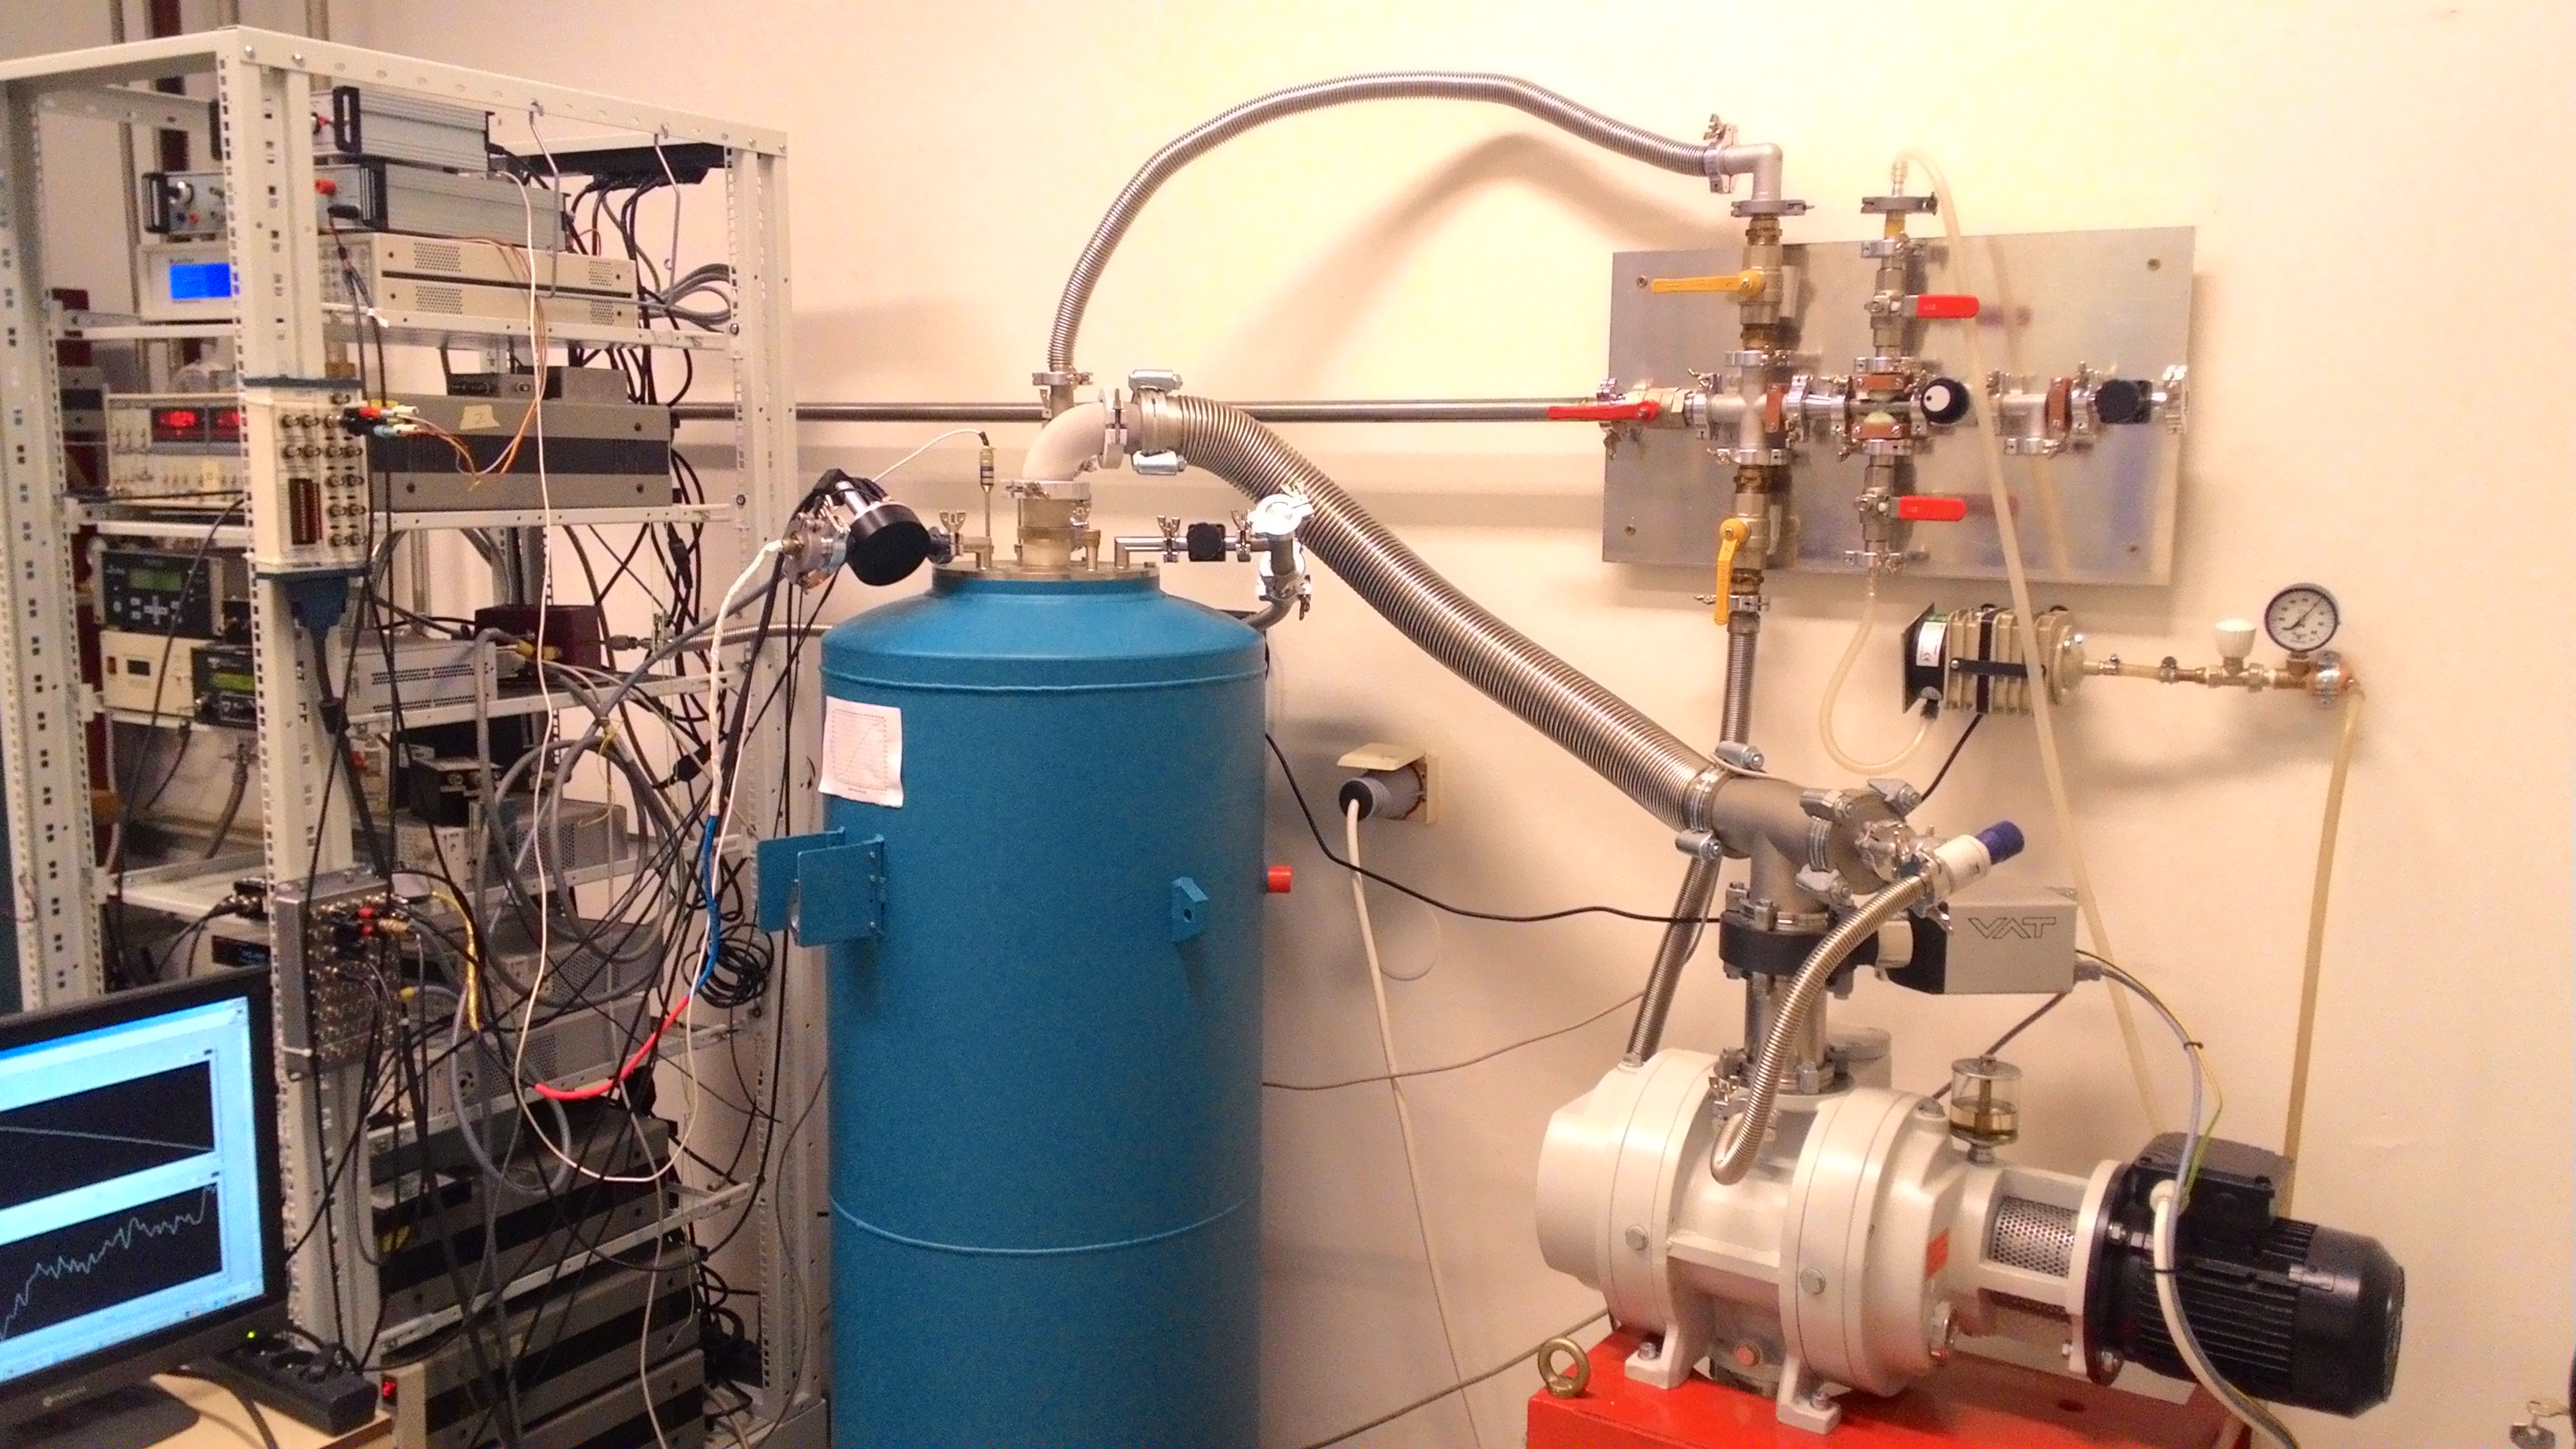
\includegraphics[width=0.9\textwidth]{graphics/exp/apparatus}
	\caption{A photograph of the experimental setup. \underline{From left}: source generators Agilent A33220, amplifying lock-ins SR830 with an I/V converters, cryostat, gas handling system (pipes) for emerging gas, rotary and Roots pump. Source: \cite{bakalaris}}
	\label{cryostat}
\end{figure}

Our chosen studied temperatures are from a wide range from a little below the transition temperature $\sim 2.17\unit{K} \gtrsim T_{\lambda}$ to the lowest (experimentally) possible one $ \sim 1.35\unit{K}$. We also performed series of measurements in the area far above the transition temperature $\sim 3 \unit{K} > T_{\lambda}$ in order to test all used components.\\
The studied range $(1.35\unit{K} - 2.17\unit{K})$ allows access to the wide range of normal/superfluid components ratios of the two-fluid model ($\rho_s / \rho_n \ll 1$ at $T\lesssim 2.17\unit{K}$ and $\rho_s / \rho_n \approx 16$ at $T\sim 1.35\unit{K}$).

Measurements at ultra-low temperatures $T < 0.6\unit{K}$ in the ballistic regime of Helium-II were performed on a Leiden Cryogenics MNK126-400 dilution refrigerator with a base temperature below $10 \unit{mK}$. The description of sub-Kelvin measurements is not included in this chapter, but is discussed in sufficient detail in \cite{universal_scaling}. However, refrigerator results are analyzed in the last section of \textbf{Results} chapter in order to test the validity of the \textit{uniform scaling} concept, introduced in the last section of the \textbf{Theoretical Background}.

\newpage

The tuning fork oscillators were tightly attached in the inner space of the cylindrical \textit{second-sound resonator} cavity, also capable to produce the second sound on the one side and receive it on the other side. We drilled a small hole to the resonator body in order to fill it with Helium-II.

This resonator (\textbf{Figure \ref{resonator}}) was  was attached at the bottom  of the \textit{insert} - a large metallic construction holding all measuring micro-devices, thermometers and coaxial cables.

\begin{figure}[h]
	\centering
	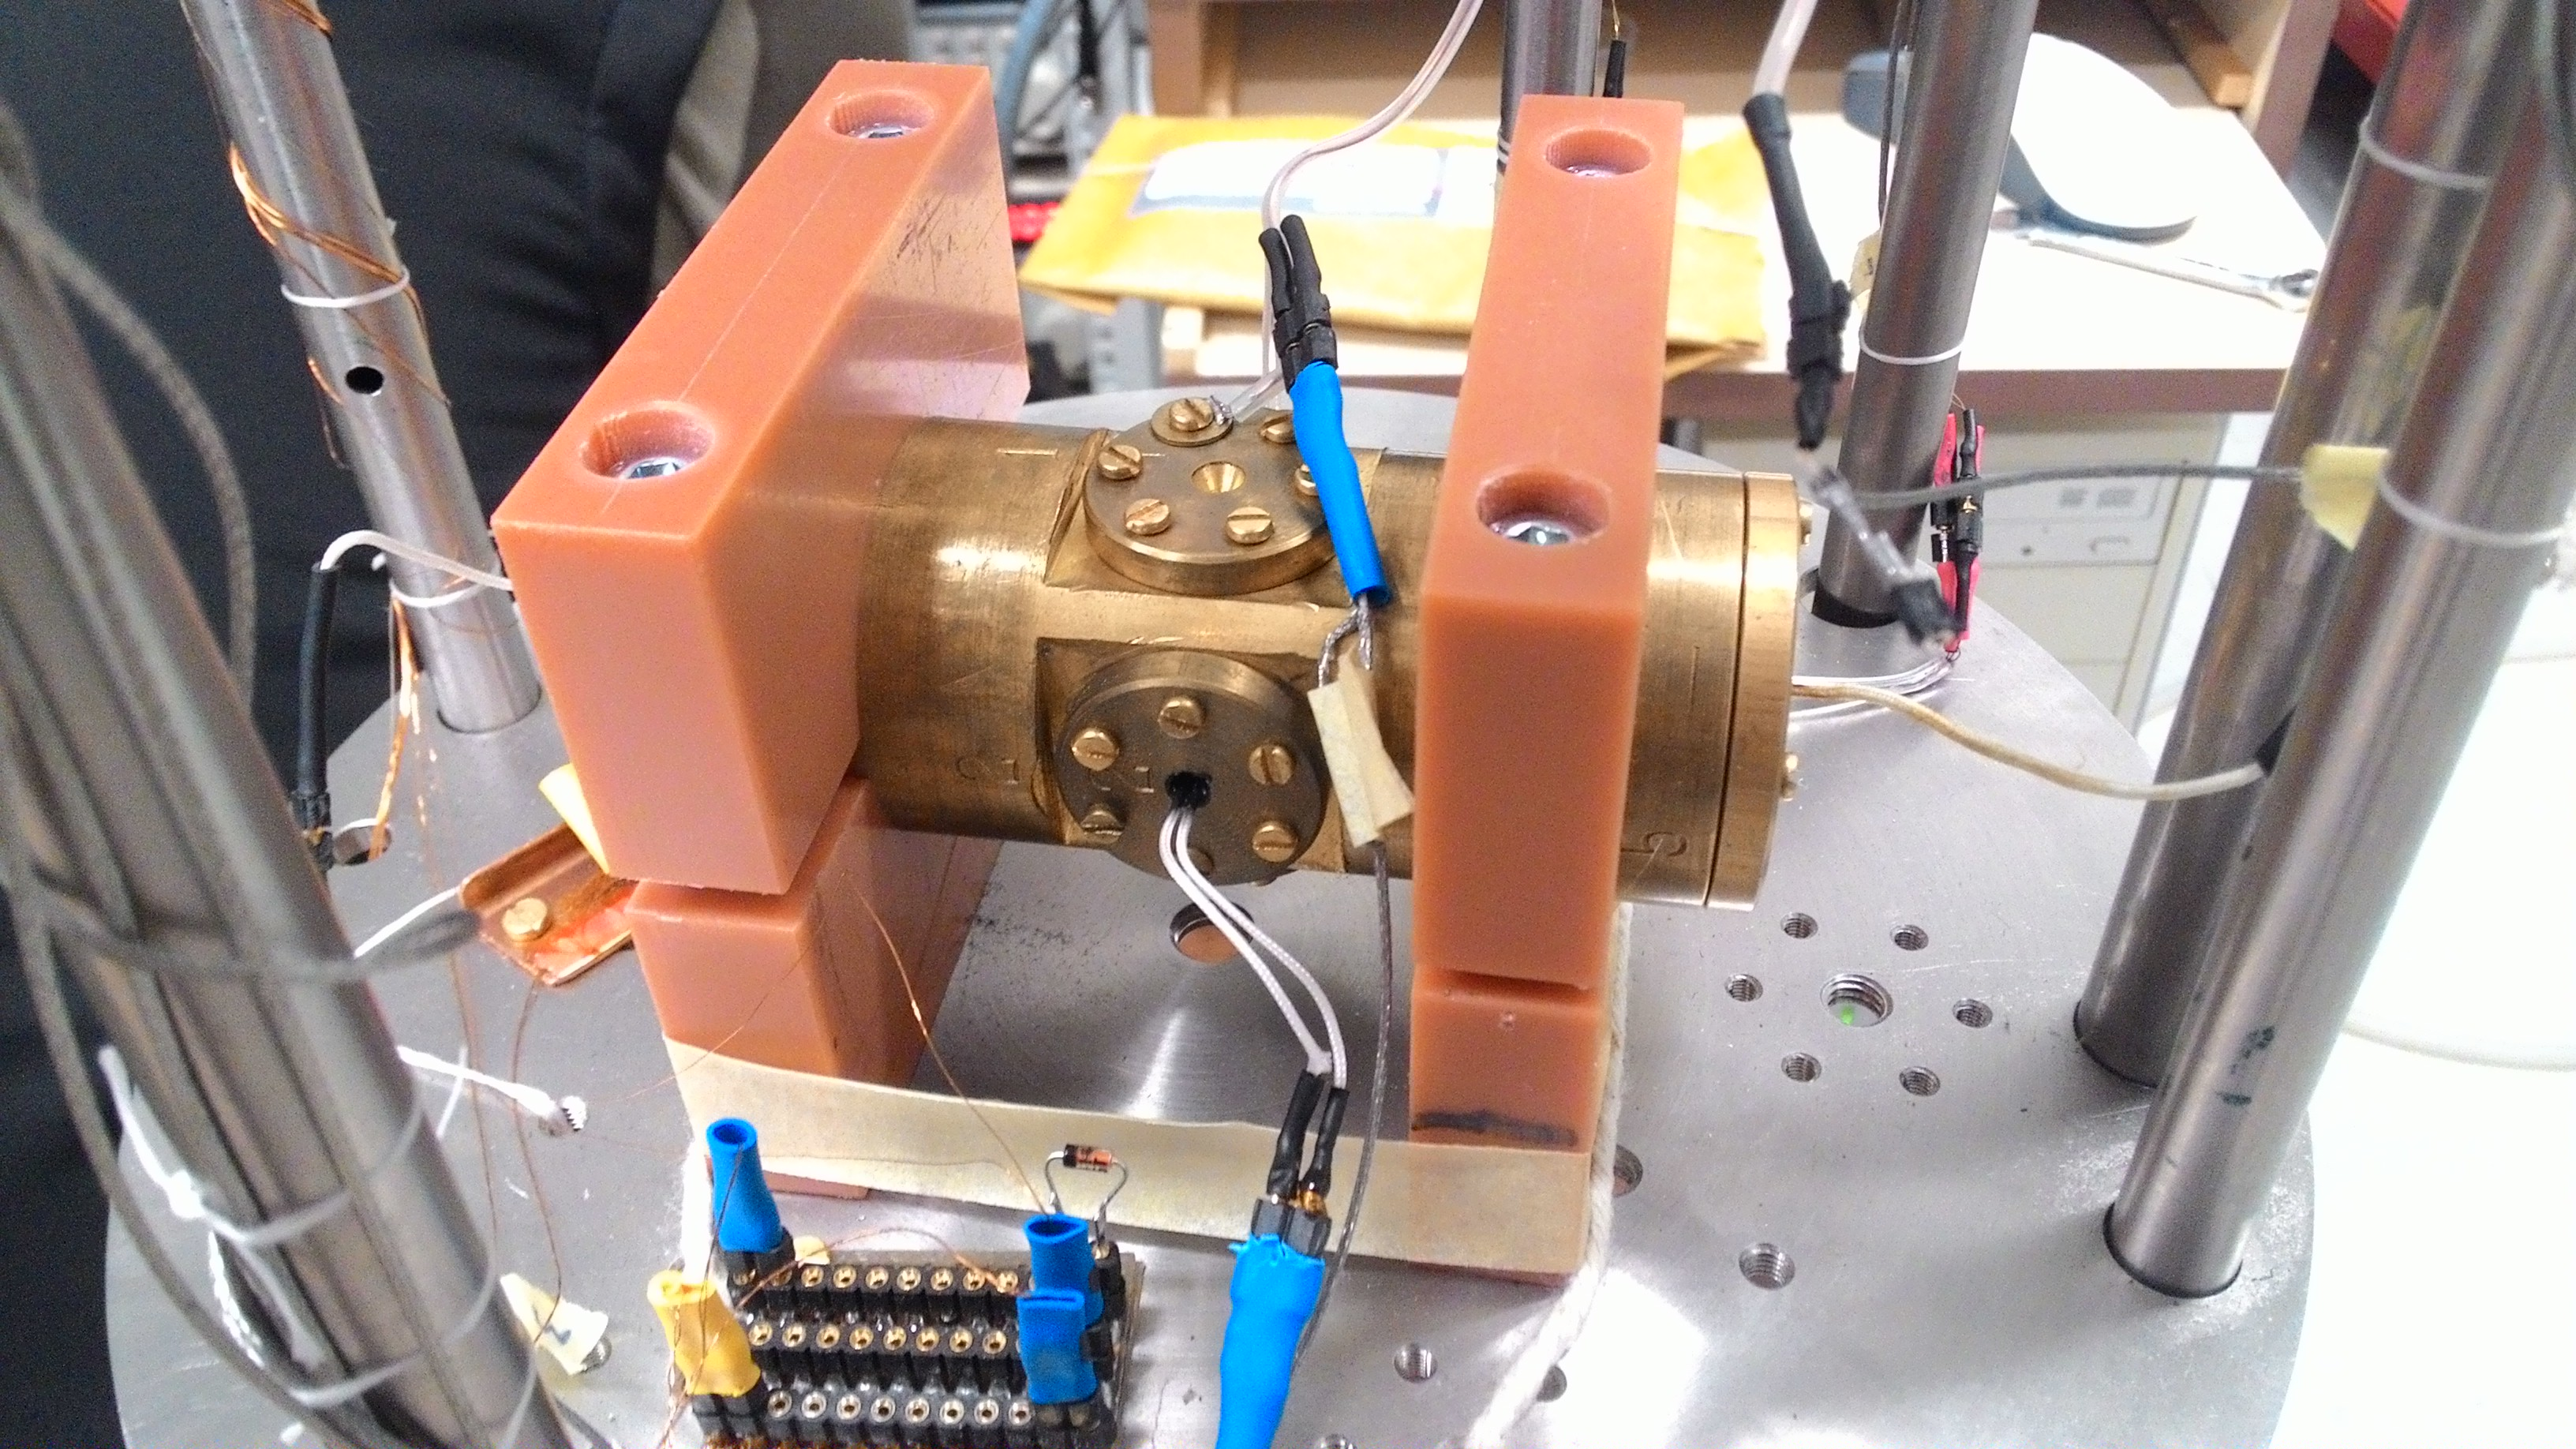
\includegraphics[width=0.9\textwidth]{graphics/exp/chamber}
	\caption{A photograph of the second-sound resonator attached at the bottom of metallic insert with cables and thermometers. Source: \cite{bakalaris}}
	\label{resonator}
\end{figure}

To obtain the best results at low temperatures, the cryostat containing oscillators was repeatedly flushed with pure liquid $\He$ from Dewar transport container. After this pre-cooling step, the liquid $\He$ was transferred using a siphon.

The inner space of resonator was additionally separated from the outer part (cryostat body) by a sintered copper, forming a solid mass of material by pressure. This ensures that no parasitic helium ices micro-particles or other impurities will interfere with the oscillators inside of resonator.


\newpage

\section{Resonators}

In this section we briefly describe the principles of micro-scale oscillators used in experiments with Helium-II.

\subsection{Vibrating Wire}

Vibrating NbTi wire resonator consists of a semi-circular loop of wire inserted to a vertical magnetic field $\vec{B}$, as shown in \textbf{Figure \ref{wire}}. As we turn on the alternating current flux $\vec{j} \propto e^{i\omega t}$ inside the wire, these currents forces the wire to oscillate due to Lorentz force $\vec{F}_L \propto \vec{j} \times \vec{B} $. As the wire moves through the field, the Faraday voltage is induced of magnitude \cite{wire}:

\begin{equation}
V = - \frac{\text{d} (\vec{B} \dotprod \vec{S})}{\text{d} t}
\sim \frac{\pi}{4} BDU\,,
\end{equation}

where $\vec{S}$ is the area vector, enclosed by the wire loop and $D$ is the distance between wire's legs. Experimentally used magnetic field was about $\approx 170 \unit{mT}$ with an uncertainty of $\pm 10 \unit{mT}$.

\begin{figure}[h]
	\centering
	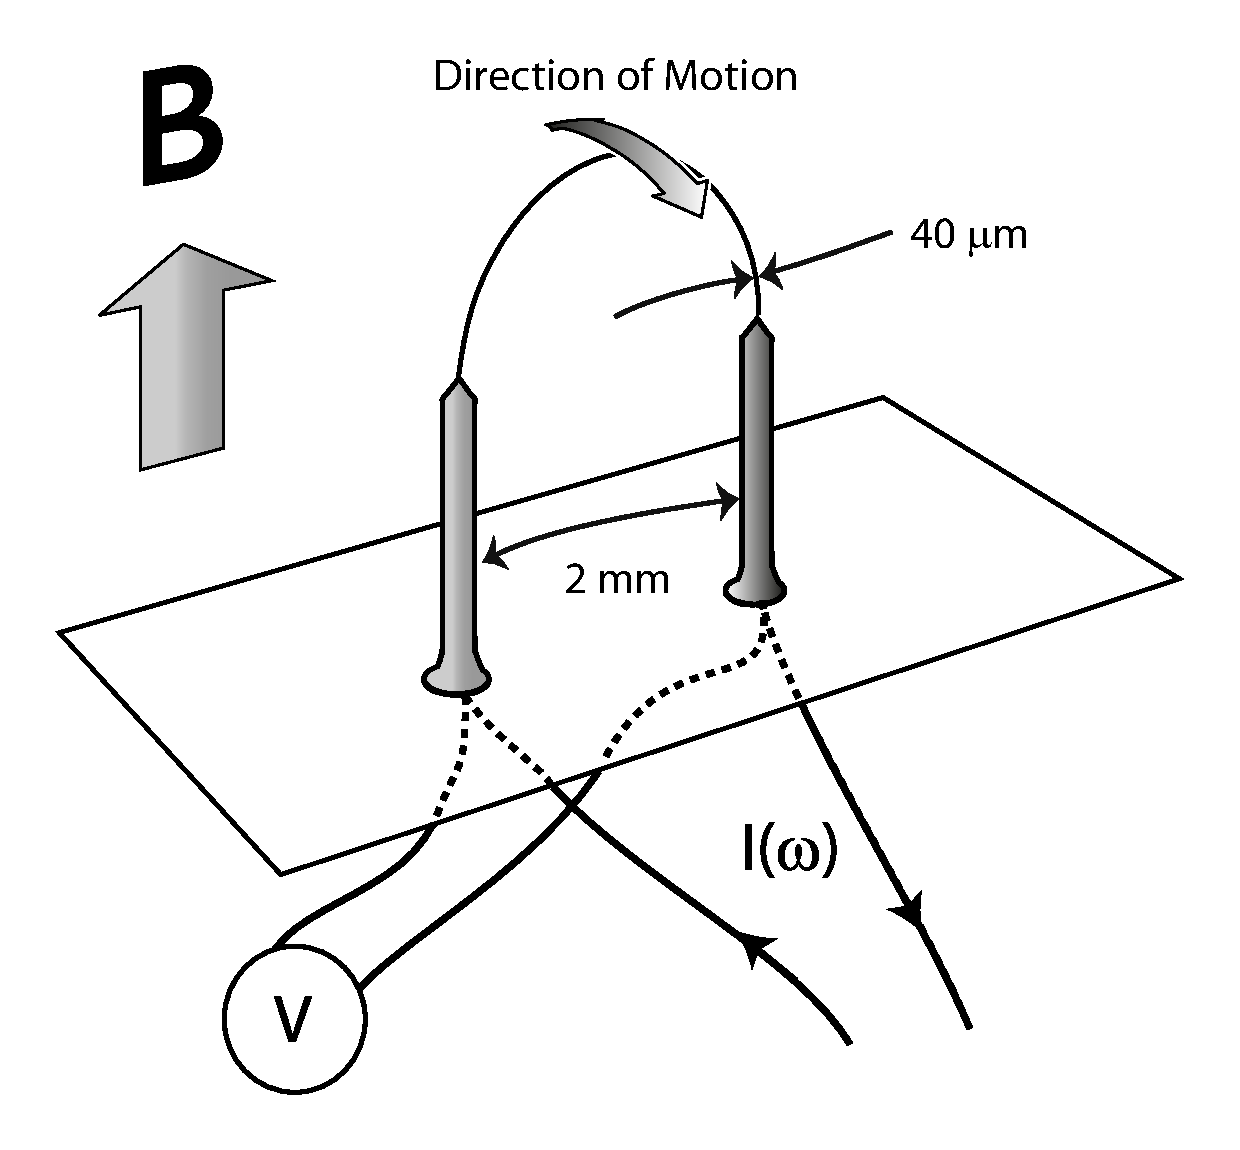
\includegraphics[width=0.5\textwidth]{graphics/exp/wire}
	\caption{Schematic diagram of the vibrating wire resonator. Source: \cite{universal_scaling}}
	\label{wire}
\end{figure}

\newpage

\subsection{Oscillating Disc}

The torsional oscillator consists of a $50 \mu\text{m}$ wire  with a glass disc fixed to
the wire at its midpoint. The disc is $1\unit{mm}$ thick with a diameter of $40\unit{mm}$. A schematics is sketched in \textbf{Figure \ref{disc}}.\\
Sixteen black marks around the circumference of the disc are used to determine the deflection and angular velocity of the disc from recorded video sequences.

\begin{figure}[h]
	\centering
	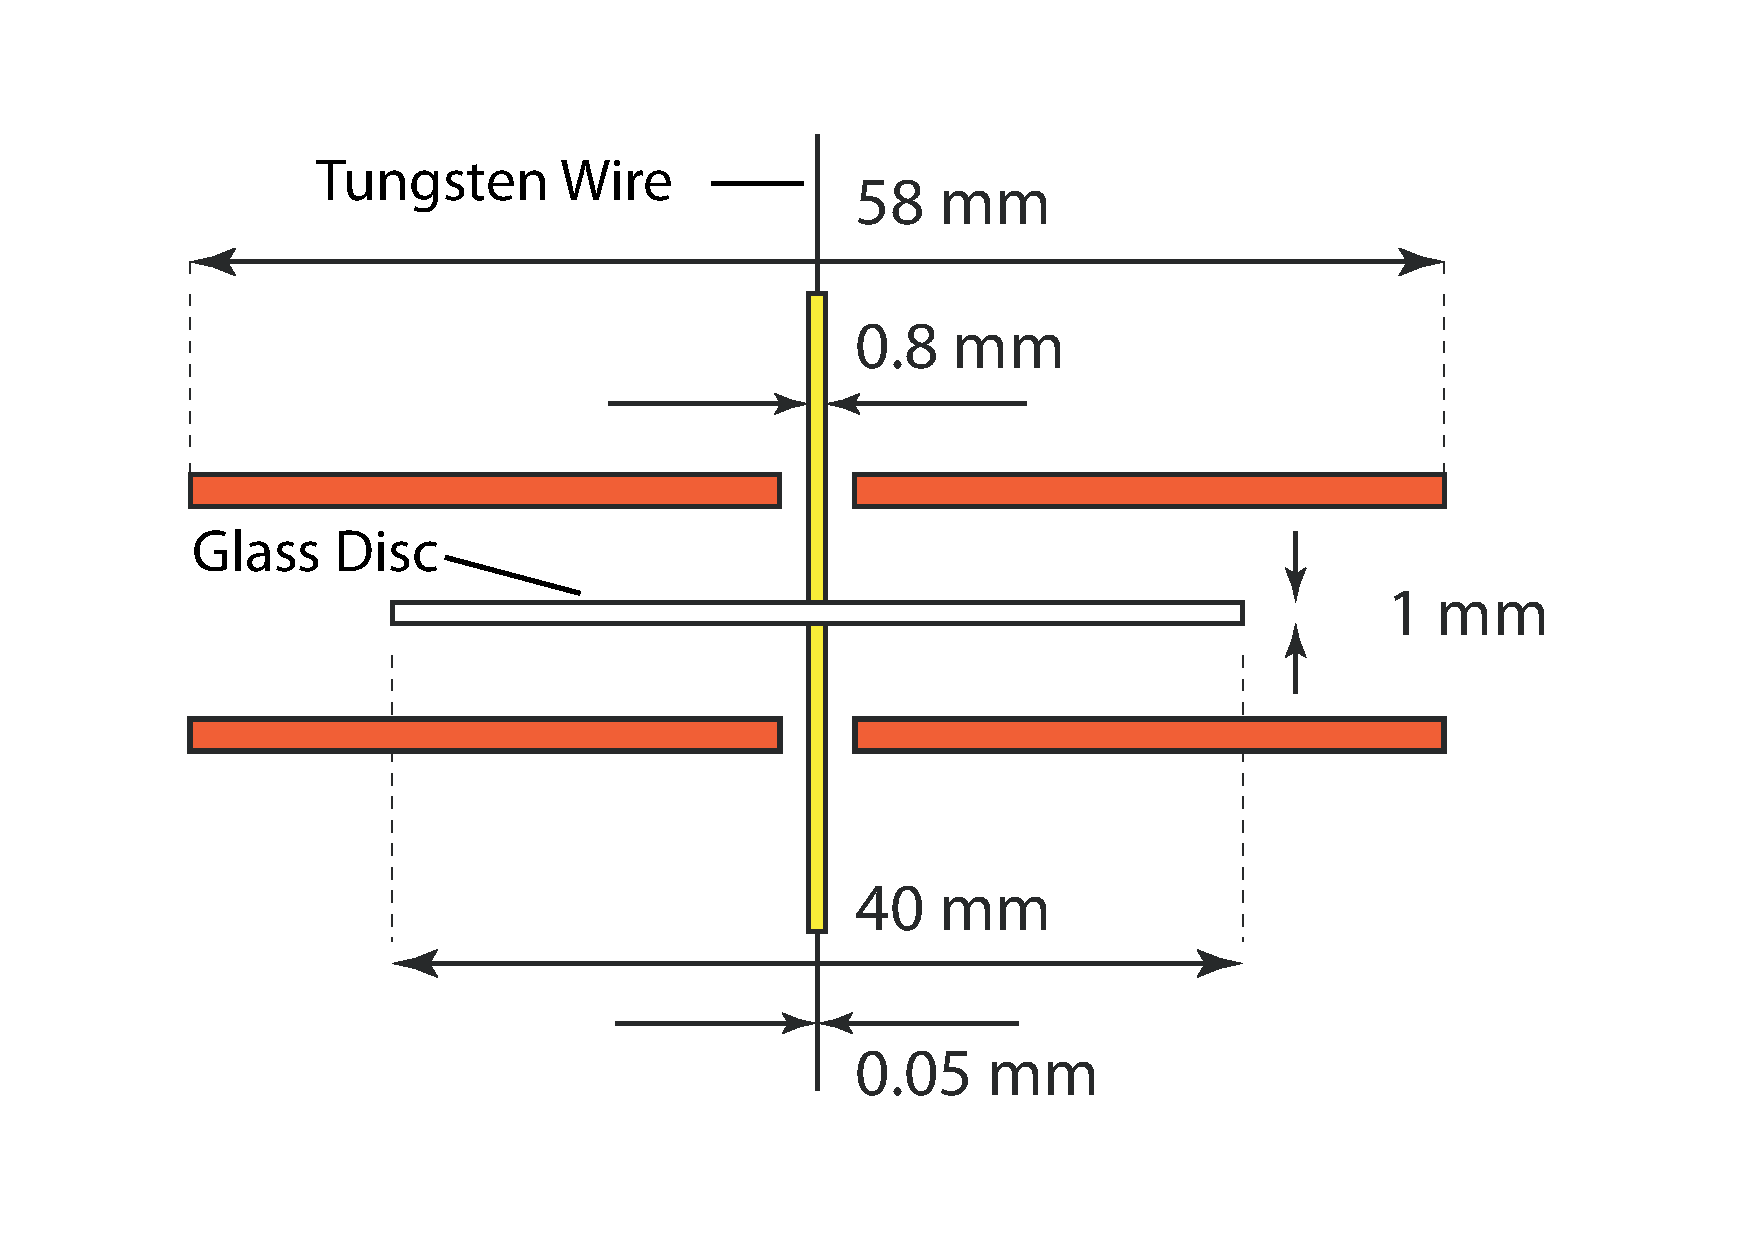
\includegraphics[width=0.7\textwidth]{graphics/exp/disc}
	\caption{Schematic diagram of the torsionally oscillating disc. Source: \cite{universal_scaling}}
	\label{disc}
\end{figure}

The raw data is in the form of video recordings of the disc motion and fairly complex post-processing method was required to extract quantities. The optical distortion from the lenses and the curved walls of the cryostat are negligible. More details about data processing can be found in \cite{universal_scaling}.

\subsection{Tuning Fork}

Quartz tuning forks (TF) are commercial piezoelectric oscillators with a well-calibrated resonant frequency. They are usually used as frequency standards in watches or as force sensors in microscopes. Also, TFs have started to be widely used in cryogenic Helium II experiments \cite{forks}.

In our experimental setup, we used the fork of following dimensions: prongs length $ \mathcal{L} = 3.50\unit{mm} $, prongs width (perpendicular to the fork plane) $ \mathcal{W}=75 \mu\unit{m} $, thickness $ \mathcal{T}=90\mu\text{m} $ prongs inter-distance $ \mathcal{D}=90\mu\text{m} $.
The same type of fork was also used and discussed in \cite{fork-exp} \cite{multiple-vels} A sketch of the fork architecture is depicted in \textbf{Figure \ref{fork}}:

\begin{figure}[h]
	\centering
	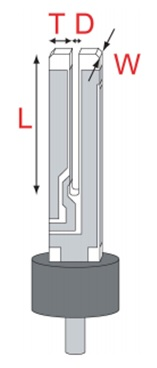
\includegraphics[width=0.2\textwidth]{graphics/exp/quartz}
	\caption{Schematic diagram of the quartz tuning fork. Source: \cite{bakalaris}}
	\label{fork}
\end{figure}

There are several achievable resonant modes at which the fork can oscillate. We chose to work with the \textit{fundamental} one at $f_0 \sim 6400 \unit{Hz}$ and with the first \textit{overtone} one at $f_1 \sim 40\,200 \unit{Hz}$.\\
The fork is driven by applying an alternating voltage $V(t) \propto e^{i\omega t}$ from a generator to the metallic plates (deposited on fork surface). The piezoelectric effect causes a tension resulting in a force, which is proportional to the applied voltage. In fundamental mode, the fork exhibits an anti-phase oscillating motion of its prongs with a single node. In case of overtone, there would be just two nodes. The fork's bend induces a piezoelectric current $I(t)$ which is proportional to the velocity $U(t)$.

The conversion relations between applied $V(t)$, measured $I(t)$ and mechanical properties $F(t)$, $U(t)$ are given \cite{forks} as:

\begin{equation}
F(t) = \frac{1}{2} a_{f} V(t)\,,
\hspace{1cm}
U(t) = \frac{I(t)}{a_{f}}\,,
\label{fork_conversions}
\end{equation}

where $a_{f}$ is the so-called \textit{fork constant}. This constant can be derived from a fork's geometry, material properties and its oscillation mode. The formula the fork constant calculation is given usually by a deflection measurement:

\begin{equation}
a_{f} = \sqrt{4\pi m_{eff} \Delta f \frac{I}{V}}\,,
\end{equation}

where $m_{eff} = TWL\rho_q /4$ ($\rho_q$ as the quartz density) is the fork's effective mass and $\Delta f$ is the measured peak width from the frequency-sweep deflection measurement. In our case we used fork with the effective mass and fork constants for fundamental and overtone mode of following values:

\begin{equation}
m_{eff} = 1.52 \times 10^{-8} \unit{kg}\,,
\hspace{7mm}
a_{f0} = 3.665 \times 10^{-7} \unit{Cm}^{-1}\,,
\hspace{7mm}
a_{f1} = 14.094 \times 10^{-7} \unit{Cm}^{-1}
\end{equation}

The measurement scheme of the experiment with tuning fork is shown in \textbf{Figure \ref{setup}}. The arrangement of experiments using dilution refrigerator were slightly more complex and are described in \cite{skyba} .

\begin{figure}[h]
	\centering
	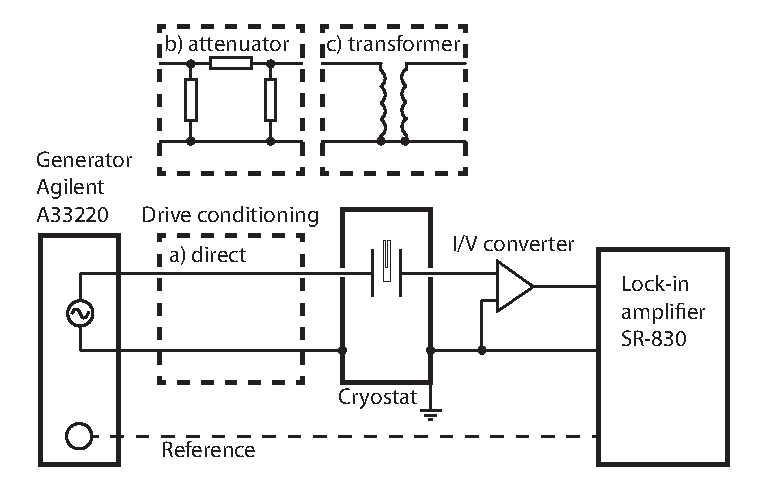
\includegraphics[width=0.6\textwidth]{graphics/exp/fork_setup}
	\caption{Diagram of the measurement scheme used in Prague. To achieve the full range of velocities, the applied voltage was either (a) directly fed to the tuning fork, (b) attenuated by one or more in-line attenuators, or (c) amplified by a transformer. The transformer’s output was constantly monitored by a Keithley digital multimeter Model 2100. The I/V converter is detailed in \cite{holt} Source:\cite{multiple-vels}}
	\label{setup}
\end{figure}

\section{Measurement technique}

It was shown in previous works \cite{svoc2016} \cite{fork-exp}  with tuning forks submerged in Helium-II that it is important to perform full \textit{frequency sweeps} across the resonant response of an oscillator in order to reveal relevant details about any nonlinear effects.\\
However, these frequency sweeps, at fixed source drive, are heavily time-consuming and sometimes it is useful (especially when we are confident about present laminar mode) to use an \textit{amplitude sweep} with changing drives, a fixed resonant frequency.\\
Since many hydrodynamic features could be overlooked by using pure amplitude sweeps, we therefore focus in our analysis mainly on the frequency sweeps.


\newpage
